\section{Scattering di Coulomb per particella di spin 0}
Calcoliamo ancora una volta la sezione d'urto per la diffusione Coulombiana questa volta utilizzando la teoria quantistica dei campi. La Lagrangiana del campo complesso di Klein-Gordon è
$$
\hat{\mathcal{L}}_0 = (\partial_\mu \hat{\phi})^\dagger (\partial_\mu \hat{\phi}) - m^2 \hat{\phi}^\dagger \hat{\phi}
$$
L'introduzione dell'interazione elettromagnetica porta al termine di interazione
$$
\hat{\mathcal{L}}' = -ie [\hat{\phi}^\dagger (\partial^\mu \hat{\phi}) - (\partial^\mu \hat{\phi}^\dagger) \hat{\phi}] A_\mu + e^2 A^\mu A_\mu \hat{\phi}^\dagger \hat{\phi}
$$
Nel seguito faremo un calcolo perturbativo al primo ordine e quindi trascuriamo il termine porporzionale a $e^2$. Abbiamo bisogno l'Hamiltoniana di interazione. Trascurando il termine $e^2$, nonostante $\mathcal{L'}$ contenga derivate di $\psi$ si trova
$$
\hat{H} = \sum_i \frac{\partial \hat{\mathcal{L}}}{\partial(\partial_0 \hat{\phi}_i)} \partial_0 \hat{\phi}_i - \hat{\mathcal{L}} \qquad \hat{H}' = ie [\hat{\phi}^\dagger (\partial^\mu \hat{\phi}) - (\partial^\mu \hat{\phi}^\dagger) \hat{\phi}] A_\mu \qquad \hat{H}' = -\hat{\mathcal{L}}'
$$
In definitiva
$$
\hat{H}' = \hat{j}^\mu A_\mu \qquad \hat{j}^\mu = ie [\hat{\phi}^\dagger (\partial^\mu \hat{\phi}) - (\partial^\mu \hat{\phi}^\dagger) \hat{\phi}] \qquad \hat{H}'(t) = \int \hat{\mathcal{H}}'(x) d^3\mathbf{r}
$$
\subsection{L'elemento di Matrice S}
L'elemento di matrice che vogliamo calcolare è $S_{if}=\langle f|S|i\rangle$. Ricordiamo lo sviluppo
$$
\hat{S} = \hat{1} + \sum_{n=1}^\infty \frac{(-i)^n}{n!} \int dt_1 \int dt_2 \dots \int dt_n T[\hat{H}_I'(t_1) \hat{H}_I'(t_2) \dots \hat{H}_I'(t_n)]
$$
Approssimando al primo ordine $(i\not=f)$
$$
S_{if} \approx \langle f | \hat{1} | i \rangle - i \langle f | \int \hat{H}_I'(t) dt | i \rangle = \delta_{if} - i \langle f | \int \hat{\mathcal{H}}_I'(x) d^4x | i \rangle
$$
$$
= - i \langle f | \hat{j}^\mu(x) A_\mu(x) | i \rangle = -i \int \langle f | \hat{j}^\mu(x) | i \rangle A_\mu(x) d^4x
$$
Calcoliamo l'elemento di matrice della corrente
$$
\hat{\phi}(\mathbf{r}, t) = \int \frac{d^3\mathbf{k}}{(2\pi)^3 \sqrt{2E_k}} \left( \hat{a}_k e^{-ik\cdot x} + \hat{b}_k^\dagger e^{+ik\cdot x} \right) \qquad k_0=E_k
$$
$$
\langle f | \hat{j}^\mu(x) | i \rangle = ie \langle f | \left[ \hat{\phi}^\dagger (\partial^\mu \hat{\phi}) - (\partial^\mu \hat{\phi}^\dagger) \hat{\phi} \right] | i \rangle
$$
\begin{align*}
\langle f | \hat{j}^\mu(x) | i \rangle = ie \int &\frac{d^3\mathbf{k}_1}{(2\pi)^3 \sqrt{2E_{k_1}}} \frac{d^3\mathbf{k}_2}{(2\pi)^3 \sqrt{2E_{k_2}}} \\
\cdot \Bigg\langle f \Bigg| &\left[ (\hat{a}_{k_1}^\dagger e^{+ik_1 \cdot x} + \hat{b}_{k_1} e^{-ik_1 \cdot x}) (-ik_2^\mu e^{-ik_2 \cdot x} + ik_2^\mu e^{+ik_2 \cdot x}) \right. \\
&\left. - (ik_1^\mu e^{+ik_1 \cdot x} - ik_1^\mu e^{-ik_1 \cdot x}) (\hat{a}_{k_2} e^{-ik_2 \cdot x} + \hat{b}_{k_2}^\dagger e^{+ik_2 \cdot x}) \right] \Bigg| i \Bigg\rangle
\end{align*}
Dopo vari conti che salto: il conto si fa sempre nello stesso modo, prendiamo operatori di distruzioni e portiamo a destra mentre gli operatori di costruzione a sinistra così agisco nel vuto che annulla.
\subsection{L'elemento di matrice della corrente j}
Riepilogando
$$
\langle f | \hat{j}^\mu(x) | i \rangle = ie \int \frac{d^3\mathbf{k}_1}{(2\pi)^3 \sqrt{2E_{k_1}}} \frac{d^3\mathbf{k}_2}{(2\pi)^3 \sqrt{2E_{k_2}}} \sqrt{2E_{p_i}} \sqrt{2E_{p_f}} \langle f | A | i \rangle
$$
$$
\langle f | A | i \rangle = -i(2\pi)^6 (k_2^\mu + k_1^\mu) e^{i(k_1-k_2) \cdot x} \delta(\mathbf{k}_2 - \mathbf{p}_i) \delta(\mathbf{k}_1 - \mathbf{p}_f)
$$
Otteniamo
$$
\langle f | \hat{j}^\mu(x) | i \rangle = e(p_i^\mu + p_f^\mu) e^{i(p_f - p_i) \cdot x}
$$
Possiamo calcolare l'elemento di matrice $S$
$$
S_{fi} = \delta_{fi} - i \int \langle f | \hat{j}^\mu(x) | i \rangle A_\mu(x) d^4x
$$
Confrontando con la definizione di $A_{fi}$ $S_{fi}=\delta_{fi}+A_{fi}$ otteniamo
$$
\mathcal{A}_{fi} = -i \int \langle f | \hat{j}^\mu(x) | i \rangle A_\mu(x) d^4x = -ie(p_i^\mu + p_f^\mu) \int e^{i(p_f - p_i) \cdot x} A_\mu(x) d^4x
$$
Abbiamo ritrovato il risultato ottenuto con la meccanica quantistica relativistica
$$
M_{fi} = ie(p_i^\mu + p_f^\mu) \int d^4x e^{-i(p_i - p_f) \cdot x} A_\mu(x)
$$
\section{Interazione elettromagnetica: spin 1/2}
Nel calcolo abbiamo utilizzato l'Hamiltoniana d'interazione
$$
\hat{\mathcal{H}}' = \hat{j}^\mu A_\mu \qquad \hat{H}'(t) = \int \hat{\mathcal{H}}'(x) d^3\mathbf{r}
$$
Nel calcolo abbiamo considerato il potenziale $A^\mu$ un campo classico noto, abbiamo trattato il più semplice problema dello scattering da potenziale. Consideriamo adesso il caso in cui il campo $A^\mu$ sia quantizzato. In questo caso i processi che possono essere descritti dall'approssimazione al primo ordine devono contenere un fotone nello stato iniziale o nello stato finale. Ad esempio la particella emette (oppure assorbe) un fotone. Lo stato iniziale contiene un elettrone e lo stato finale contiene un elettrone e un fotone
$$
|i\rangle = \hat{a}_{\mathbf{p}_i, s_i}^\dagger |0\rangle
$$
$$
|f\rangle = \hat{a}_{\mathbf{p}_f, s_f}^\dagger \hat{c}_{\mathbf{q}_f, \lambda}^\dagger |0\rangle
$$
L'elemento di matrice è
$$
\langle i | \hat{\mathcal{H}}' | f \rangle = \langle 0 | \hat{a}_{\mathbf{p}_i, s_i} \hat{j}^\mu \hat{A}_\mu \hat{a}_{\mathbf{p}_f, s_f}^\dagger \hat{c}_{\mathbf{q}_f, \lambda}^\dagger |0\rangle
$$
Gli operatori $j_\mu$ e $A_\mu$ contengono gli opportuni operatori di creazione e distruzione tali che l'elemento di matrice sia diverso da zero. Senza fotone nello stato finale l'elemento di matrice sarebbe nullo. Analogamente senza gli elettroni negli stati iniziali e finali. Ad esempio senza un fotone nello stato finale (o iniziale) l'elemento di matrice sarebbe
$$
\langle 0 | \hat{a}_{p_f} \hat{j}^\mu \hat{A}_\mu \hat{a}_{p_i}^\dagger | 0 \rangle
$$
Ricordiamo lo sviluppo di $A^\mu$
$$
\hat{A}^\mu(x) = \sum_{\lambda=1,2} \int \frac{d^3\mathbf{k}}{(2\pi)^3 \sqrt{2|\mathbf{k}|}} \left( \epsilon^\mu_{\mathbf{k},\lambda} \hat{c}_{\mathbf{k},\lambda} e^{-ik\cdot x} + \epsilon^{\mu *}_{\mathbf{k},\lambda} \hat{c}_{\mathbf{k},\lambda}^\dagger e^{+ik\cdot x} \right)
$$
Sviluppando l'elemento di matrice come abbiamo fatto per lo scattering da potenziale gli operatori $c$ possono essere portati a destra e danno contributo nullo, gli operatori $c^\dagger$ possono essere portati a dinistra e danno contributo nullo. Concludiamo che se lo stato iniziale o finale non contengono un fotone l'elemento di matrice è nullo. Tuttavia il processo appena descritto non è cinematicamente permesso. Infatti, se la particella iniziale e finale coincidono il processo con un fotone reale non è possibile perchè violerebbe la conservazione del $4-$momento.
$$
p_i=p_f\pm q
$$
Il segno $\pm$ si riferisce alla emissione o all'assorbimento di un fotone rispettivamente. Elevando al quadrato ambo i membri (ricordando che per un fotone reale si ha $q^2=0$)
$$
m^2=m^2\pm p\cdot q \quad \Longrightarrow \quad p_f\cdot q=0
$$
Sviluppando il prodotto scalare nel sistema di riposo dell'elettrone finale ($p_f$) abbiamo pertanto
$$
mE_q=0 \qquad E_q=|\mathbf{q}|=0
$$
Vediamo pertanto che la reazione in esame è possibile solo per un fotone reale di energia nulla. Notiamo, tuttavia, che sarebbe possibile per un fotone virtuale ($q^2\not=0$). Concludiamo che il primo termine non nullo dello sviluppo perturbativo è del secondo ordine
$$
\hat{S} = \hat{1} - \frac{1}{2} \iint d^4x_1 d^4x_2 T[\hat{\mathcal{H}}'_I(x_1) \hat{\mathcal{H}}'_I(x_2)] \qquad \hat{\mathcal{H}}'_I = \hat{j}^\mu \hat{A}_\mu
$$
nel calcolo dell'elemento di matrice per un processo 
\begin{figure}[h!]
    \centering
    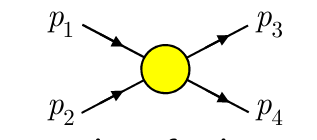
\includegraphics[width=0.6\textwidth]{Lezioni/Lezione 10/ik.png}
    \label{fig:ik}
\end{figure}
Abbiamo i seguenti stati iniziale e finale
$$
|i\rangle = |\mathbf{p}_1, \mathbf{p}_2\rangle = \hat{a}_{\mathbf{p}_1}^\dagger \hat{a}_{\mathbf{p}_2}^\dagger |0\rangle \qquad |f\rangle = |\mathbf{p}_3, \mathbf{p}_4\rangle = \hat{a}_{\mathbf{p}_3}^\dagger \hat{a}_{\mathbf{p}_4}^\dagger |0\rangle
$$
Dobbiamo pertanto calcolare
$$
\langle 0 | \hat{a}_{\mathbf{p}_3} \hat{a}_{\mathbf{p}_4} T[\hat{\mathcal{H}}'_I(x_1) \hat{\mathcal{H}}'_I(x_2)] \hat{a}_{\mathbf{p}_1}^\dagger \hat{a}_{\mathbf{p}_2}^\dagger |0\rangle
$$
In forma più estesa
$$
\langle 0 | \hat{a}_{\mathbf{p}_3} \hat{a}_{\mathbf{p}_4} T[\hat{j}^\mu(x_1) \hat{A}_\mu(x_1) \hat{j}^\mu(x_2) \hat{A}_\mu(x_2)] \hat{a}_{\mathbf{p}_1}^\dagger \hat{a}_{\mathbf{p}_2}^\dagger |0\rangle
$$
Non calcoleremo nel dettaglio l'elemento di matrice ma faremo delle considerazioni generali. Innanzitutto, dal momento che i campi del fotone e dei fermioni commutano
$$
[\hat{A}^\mu, \hat{j}^\nu] = 0
$$
$$
T[\hat{j}^\mu(x_1)\hat{A}_\mu(x_1)\hat{j}^\nu(x_2)\hat{A}_\nu(x_2)] = T[\hat{j}^\mu(x_1)\hat{j}^\nu(x_2)]T[\hat{A}_\mu(x_1)\hat{A}_\nu(x_2)]
$$
Nel caso del processo che stiamo esaminando non ci sono fotoni negli stati iniziale e finale. I campi fotonici agiscono direttamente sugli stati di vuoto
$$
|0\rangle \equiv |0,e\rangle_{k_1} \otimes |0,\gamma\rangle_{k_2} \otimes \dots
$$
Possiamo quindi fattorizzare l'elemento di matrice
$$
\langle 0 | \hat{a}_{\mathbf{p}_3} \hat{a}_{\mathbf{p}_4} T[\hat{j}^\mu(x_1) \hat{j}^\nu(x_2)] \hat{a}_{\mathbf{p}_1}^\dagger \hat{a}_{\mathbf{p}_2}^\dagger |0\rangle \langle 0 | T[\hat{A}_\mu(x_1) \hat{A}_\nu(x_2)] |0\rangle
$$
Si definisce propagatore fotonico l'espressione
$$
D_{\mu\nu}(x_1, x_2) = i \langle 0 | T[\hat{A}_\mu(x_1) \hat{A}_\nu(x_2)] |0\rangle
$$
Graficamente viene rappresentato così
\begin{figure}[h!]
    \centering
    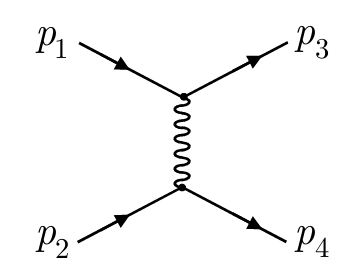
\includegraphics[width=0.4\textwidth]{Lezioni/Lezione 10/fe.png}
    \label{fig:fe}
\end{figure}
Si può dimostrare che il propagatore dipende solo dalla differenza delle coordinate $x_1$ e $x_2$
$$
D_{\mu\nu}(x_1, x_2) = D_{\mu\nu}(x_1 - x_2)
$$
Il propagatore è la funzione di Green dell'equazione del campo elettromagnetico (equazione dell'onda elettromagnetica)
$$
\Box D_{\mu\nu}(x_1 - x_2) = g_{\mu\nu} \delta^4(x_1 - x_2)
$$
La forma esplicita 
$$
D_{\mu\nu}(x - x') = \frac{1}{4\pi} \frac{g_{\mu\nu}}{|\mathbf{r} - \mathbf{r}'|} \delta\left[ c \left( t - t' - \frac{|\mathbf{r} - \mathbf{r}'|}{c} \right) \right]
$$
La sua trasformata di Fourier è
$$
\tilde{D}_{\mu\nu}(q) = - \frac{g_{\mu\nu}}{q^2}
$$
Ritorneremo presto su questo propagatore. Consideriamo adesso la parte dell'elemento di matrice relativa ai fermioni
$$
\langle 0 | \hat{a}_{\mathbf{p}_3} \hat{a}_{\mathbf{p}_4} T[\hat{j}^\mu(x_1) \hat{j}^\nu(x_2)] \hat{a}_{\mathbf{p}_1}^\dagger \hat{a}_{\mathbf{p}_2}^\dagger | 0 \rangle
$$
Occorrerebbe trattare attentamente l'eventualità di particelle identiche ,a per questi calcoli sono statte messe a punto tecniche molto efficaci. In particolare la contrazione di operatori di campo, il teorema di Wick e le regole di Feynman. Ai nostri fini diciamo che per particelle non identiche (esempio scattering elettrone-protone) l'elemento di matrice si fattorizza in due pezzi
$$
\langle 0 | \hat{a}_{\mathbf{p}_3} \hat{j}^\mu(x_1) \hat{a}_{\mathbf{p}_1}^\dagger | 0 \rangle \langle 0 | \hat{a}_{\mathbf{p}_4} \hat{j}^\nu(x_2) \hat{a}_{\mathbf{p}_2}^\dagger | 0 \rangle
$$
Infine (faremo il calcolo in seguito)
$$
\langle 0 | \hat{a}_{\mathbf{p}_3} \hat{j}^\mu(x_1) \hat{a}_{\mathbf{p}_1}^\dagger | 0 \rangle = -e \overline{u}_{\mathbf{p}_3, s_3} \gamma^\mu u_{\mathbf{p}_1, s_1} e^{-i(p_1-p_3) \cdot x_1}
$$
$$
\langle 0 | \hat{a}_{\mathbf{p}_4} \hat{j}^\nu(x_2) \hat{a}_{\mathbf{p}_2}^\dagger | 0 \rangle = -e \overline{u}_{\mathbf{p}_4, s_4} \gamma^\nu u_{\mathbf{p}_2, s_2} e^{-i(p_2-p_4) \cdot x_2}
$$
Notiamo che abbiamo ritrovato la forma delle correnti di transizione dell'equazione di Dirac. Ricordiamo l'espressione per la matrice $S$ al secondo ordine
$$
\hat{S} = \hat{1} - \frac{1}{2} \iint d^4x_1 d^4x_2 T[\hat{\mathcal{H}}'_I(x_1) \hat{\mathcal{H}}'_I(x_2)]
$$
occorre integrare su $x_1$ e $x_2$, inoltre $S_{fi}=\delta_{fi}+A_{fi}$. Pertanto
$$
\mathcal{A}_{fi} = -\frac{1}{2} \iint d^4x_1 d^4x_2 \hat{j}_1^\mu(x_1) D_{\mu\nu}(x_1 - x_2) \hat{j}_2^\nu(x_2)
$$
La corrente $j_1(x_1)$ interagisce con $A_\mu$ nel punto dello spazio-tempo $x_1$. Il propagatore $D_{\mu\nu}(x_1-x_2)$ propaga l'interazione da $x_1$ a $x_2$. La corrente $j_2(x_2)$ interagisce con $A_\mu$ nel punto dello spazio tempo $x_2$. Passiamo nello spazio dei moenti e facciamo un cambio di variabile
$$
x_1 - x_2 = z \qquad x_2 = x_1 - z \qquad dx_2 = -dz
$$
$$
x_1 = x \qquad \mathcal{A}_{fi} = \frac{1}{2} \int d^4x d^4z \, \hat{j}_1^\mu(x) D_{\mu\nu}(z) \hat{j}_2^\nu(x - z)
$$
Ricordiamo il risultato trovato per gli elementi di matrice delle correnti 
$$
\hat{j}_1^\mu(x_1) = -e \overline{u}_{\mathbf{p}_3, s_3} \gamma^\mu u_{\mathbf{p}_1, s_1} e^{-i(p_1-p_3) \cdot x_1} \qquad \hat{j}_2^\nu(x_2) = -e \overline{u}_{\mathbf{p}_4, s_4} \gamma^\nu u_{\mathbf{p}_2, s_2} e^{-i(p_2-p_4) \cdot x_2}
$$
E otteniamo $(u_{\mathbf{p}\alpha, s_\alpha} \to u_\alpha, \alpha = 1,2,3,4)$
$$
\mathcal{A}_{fi} = \frac{1}{2} e^2 \overline{u}_3 \gamma^\mu u_1 \overline{u}_4 \gamma^\nu u_2 \int d^4x d^4z e^{-i(p_1-p_3) \cdot x} D_{\mu\nu}(z) e^{-i(p_2-p_4) \cdot (x-z)}
$$
Otteniamo pertanto
$$
M_{fi} = \frac{e^2}{2} \overline{u}_3 \gamma^\mu u_1 \overline{u}_4 \gamma^\nu u_2 \int d^4x e^{-i(p_1-p_3+p_2-p_4) \cdot x} \int d^4z D_{\mu\nu}(z) e^{-i(p_4-p_2)z} \quad q = p_4 - p_2
$$
Le parti evidenziate sono rispettivamente: la funzione $\delta()$ e la trasformata di Fourier del propagatore (o Funzione di Green). Abbiamo definitivamente
$$
\mathcal{A}_{fi} = \frac{e^2}{2} \overline{u}_3 \gamma^\mu u_1 \overline{u}_4 \gamma^\nu u_2 (2\pi)^4 \delta(p_1 - p_3 + p_2 - p_4) \tilde{D}_{\mu\nu}(q)
$$
Abbiamo definito il $4-$momento trasferito
$$
q = p_1 - p_3 = p_4 - p_2
$$
Inoltre ricordiamo che
$$ 
\tilde{D}_{\mu\nu}(q) = - \frac{g_{\mu\nu}}{q^2} \qquad \mathcal{A}_{fi} = i (2\pi)^4 \delta^4(p_1 + p_2 - p_3 + p_4) \mathfrak{M}_{fi}
$$
Per finire
$$
\mathfrak{M}_{fi} = -i \frac{e^2}{2} \overline{u}_3 \gamma^\mu u_1 \frac{g_{\mu\nu}}{q^2} \overline{u}_4 \gamma^\nu u_2
$$
\section{Regole di Feynman}
Diamo le regole di Feynman per l'ordine perturbativo più basso. Il cosiddetto tree-level (livello d'albero, quindi non ci sono loop). In un diagramma ci sono linee esterne e linee interne:
\begin{itemize}
    \item Le linee esterne corrispondono alle particelle negli stati iniziale e finale (particelle reali)
    \item Le linee interne corrispondono a stati virtuali tramite i quali descrivono l'interazione (particelle virtuali, propagatori)
\end{itemize}
Per ogni elemento occorre introdurre un fattore (funzione) nella ampiezza $-i\mathfrak{M}$
\begin{figure}[h!]
    \centering
    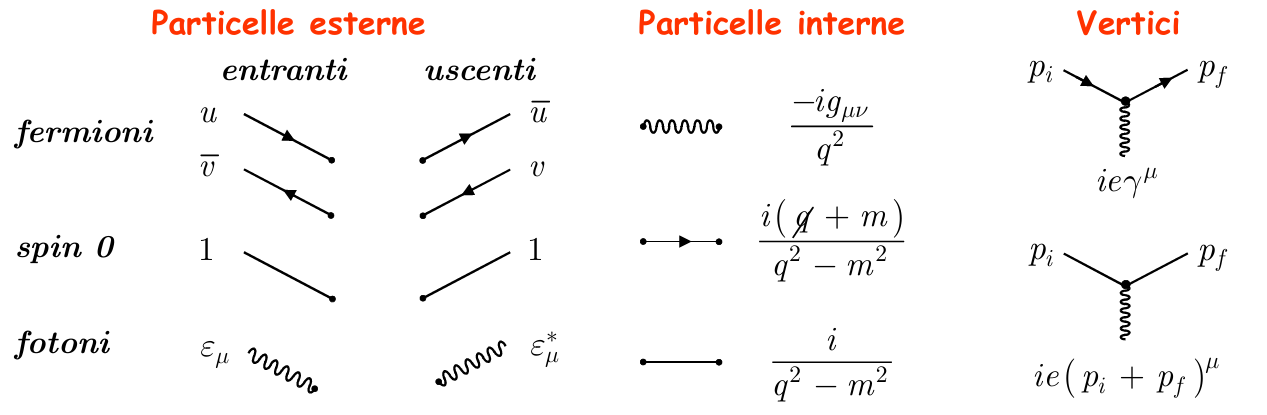
\includegraphics[width=0.9\textwidth]{Lezioni/Lezione 10/fer.png}
    \label{fig:fer}
\end{figure}
Come si può notare tutti i propagatori hanno una divergenza che corrisponde alla massa del propagatore. Per quanto riguarda il fotone la massa è nulla.
\section{Sezione d'urto elettrone-muone}
Calcoliamo adesso la sezione d'urto del processo $e^-\mu^-\to e^-\mu^-$ utilizzando le regole di Feynman. Il diagramma del processo è:
\begin{itemize}
    \item Abbiamo due fermioni entranti
    \item Abbiamo due fermioni uscenti
    \item Abbiamo due vertici fermione fotone
    \item C'è un propagatore fotonico
\end{itemize}
\begin{figure}[h!]
    \centering
    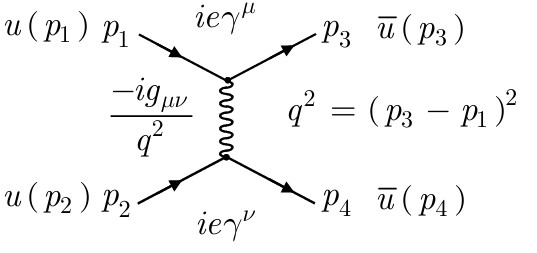
\includegraphics[width=0.6\textwidth]{Lezioni/Lezione 10/red.png}
    \label{fig:red}
\end{figure}
L'ampiezza invariante è
$$
-i\mathfrak{M} = \overline{u}_3(ie\gamma^\mu)u_1 \frac{-ig_{\mu\nu}}{q^2} \overline{u}_4(ie\gamma^\nu)u_2 \qquad \mathfrak{M} = -e^2 \overline{u}_3 \gamma^\mu u_1 \frac{1}{q^2} \overline{u}_4 \gamma_\mu u_2
$$
Se fosse $e^-e^-\to e^-e^-$ ci sarebbero $2$ diagrammi (con $p_3$ e $p_4$ scambiati e un segno meno relativo). Per il calcolo di $|\mathfrak{M}|^2$ si utilizzano le tecniche di tracce delle matrici $\gamma$ sviluppate precedentemente. In particolare sappiamo che le due correnti portano a due tensori
$$
L_e^{\alpha\beta} = \frac{1}{2}Tr[(\slashed{p}_3 + m_e)\gamma^\alpha (\slashed{p}_1 + m_e)\gamma^\beta]
$$
$$
L_{\mu}^{\alpha\beta} = \frac{1}{2}Tr[(\slashed{p}_4 + m_\mu)\gamma^\alpha (\slashed{p}_2 + m_\mu)\gamma^\beta]
$$
Il calcolo dei due tensori dà
$$
L_e^{\alpha\beta} = 2[p_3^\alpha p_1^\beta + p_1^\alpha p_3^\beta - (p_1 \cdot p_3 - m_e^2)g^{\alpha\beta}]
$$
$$
L_\mu^{\alpha\beta} = 2[p_4^\alpha p_2^\beta + p_2^\alpha p_4^\beta - (p_2 \cdot p_4 - m_\mu^2)g^{\alpha\beta}]
$$
Il modulo quadrato dell'ampiezza è
$$
\overline{|\mathfrak{M}|^2} = \frac{e^4}{q^4} L_{e}^{\alpha\beta} L_{\mu,\alpha\beta}
$$
$$
= \frac{8e^4}{q^4} [(p_3 \cdot p_4)(p_1 \cdot p_2) + (p_3 \cdot p_2)(p_1 \cdot p_4) - m_e^2 p_4 \cdot p_2 - m_\mu^2 p_1 \cdot p_3 + 2m_e^2 m_\mu^2]
$$
Consideriamo il limite ultra-realtivistico (trascuriamo le masse)
$$
\overline{|\mathfrak{M}|^2} = \frac{8e^4}{q^4} [(p_3 \cdot p_4)(p_1 \cdot p_2) + (p_3 \cdot p_2)(p_1 \cdot p_4)]
$$
Ricordiamo la formula della sezione d'urto
$$
d\sigma = \frac{|\mathfrak{M}|^2}{4\sqrt{(p_1 \cdot p_2)^2 - m_1^2 m_2^2}} d\Phi_n(p_1 + p_2; p_3, \dots, p_{n+2})
$$
Calcoliamo adesso lo spazio delle fasi e il flusso incidente.
\subsection{Variabili di Mandelstam}
Consideriamo lo scattering $1+2\to3+4$ e ricordiamo la conservazione del $4-$momento
$$
p_1+p_2=p_3+p_4
$$
Definiamo le variabili di Mandelstam
$$
s = (p_1 + p_2)^2 = (p_3 + p_4)^2 \qquad t = (p_1 - p_3)^2 = (p_4 - p_2)^2 \qquad 
$$
$$
u = (p_1 - p_4)^2 = (p_3 - p_2)^2 \qquad q^2 = (p_3 - p_1)^2 = t
$$
Specializziamo le relazioni nel centro di massa trascurando le masse delle particelle ($p^2_i=0, |\mathbf{p_i}=E_i|$)
$$
s = 2p_1 \cdot p_2 = 2p_3 \cdot p_4 \qquad \Longrightarrow\qquad  p_1 \cdot p_2 = p_3 \cdot p_4 = \frac{s}{2} = 2\mathbf{p}^2
$$
$$
t = -2p_1 \cdot p_3 = -2p_2 \cdot p_4 \qquad \Longrightarrow\qquad p_1 \cdot p_3 = p_2 \cdot p_4 = -\frac{t}{2} = \mathbf{p}^2 (1 - \cos\theta^*)
$$
$$
u = -2p_1 \cdot p_4 = -2p_2 \cdot p_3 \qquad \Longrightarrow\qquad p_1 \cdot p_4 = p_2 \cdot p_3 = -\frac{u}{2} = \mathbf{p}^2 (1 + \cos\theta^*)
$$
Calcoliamo l'elemento di matrice in funzione di $s,t,u$

\begin{align*}
\overline{|\mathfrak{M}|^2} &= \frac{8e^4}{q^4}[(p_3 \cdot p_4)(p_1 \cdot p_2) + (p_3 \cdot p_2)(p_1 \cdot p_4)]= \frac{8e^4}{t^2} \left[ \frac{s^2}{4} + \frac{u^2}{4} \right] = 2e^4 \frac{s^2 + u^2}{t^2}\\
&= 2e^4 \frac{16\mathbf{p}^4 + 4\mathbf{p}^4 (1 + \cos\theta^*)^2}{4\mathbf{p}^4 (1 - \cos\theta^*)^2} = 2e^4 \frac{16 + 16 \cos^4 \frac{\theta^*}{2}}{16 \sin^4 \frac{\theta^*}{2}} = 2e^4 \frac{1 + \cos^4 \frac{\theta^*}{2}}{\sin^4 \frac{\theta^*}{2}}
\end{align*}
\subsection{Cinematica della reazione}
Prima di iniziare il calcolo del flusso e dello spazio delle fasi discutiamo alcuni aspetti della cinematica della reazione. Analizziamo lo stato finale: abbiamo 2 particelle per un totale di $8$ variabili cinematiche. La relazione $E^2=m^2+p^2$ riduce le variabili a $6$, inoltre la conservazione dell'energia-impulso totali ($4$ relazioni) riduce ulteriormente a $2$ le variabili indipendenti. In assenza di polarizzazione nello stato iniziale una rotazione di un angolo $\phi$ intorno all'asse definito dal fascio è inessenziale. Pertanto, per descrivere lo stato finale, è sufficiente una sola variabile. Sono possibili diverse scelte, ad esempio: angolo di deflessione $\theta$, energia $E$ di una delle due particelle $3,4$ o variabile di Mandelstam $t$ (che è relativisticamente invariante)
$$
t=\left(p_3-p_1\right)^2\qquad t=m^2+m^2-2E_1E_3+2|\mathbf{p_1}||\mathbf{p}_2|\cos{\theta}
$$
Ricordiamo l'altra variabile di Mandelstam $s = (p_1 + p_2)^2 = (p_3 + p_4)^2$.
\subsection{Lo spazio delle fasi della reazione}
Calcoliamo lo spazio delle fasi per il processo $1+2\to 3+4$ o $p_1+p_2\to p_3+p_4$.
$$
d\Phi_2 = (2\pi)^4 \delta^4(p_1 + p_2 - p_3 - p_4) \frac{d^3\mathbf{p}_3}{(2\pi)^3 2E_3} \frac{d^3\mathbf{p}_4}{(2\pi)^3 2E_4}
$$
Integrando sul $3-$momento $\mathbf{p}_4$ della particella $4$
$$
d\Phi_2 = \delta(E_1 + E_2 - E_3 - E_4) \frac{(2\pi)}{2E_4} \frac{d^3\mathbf{p}_3}{(2\pi)^3 2E_3} \qquad E_4 = \sqrt{\mathbf{p}_4^2 + m_4^2}
$$
Questa formula è valida in tutti i sistemi di riferimento, specializziamo la formula nel sistema del centro di massa $\mathbf{p}_3=-\mathbf{p}_4\equiv \mathbf{q}_f$
$$
E_3^2 = \mathbf{q}_f^2 + m_3^2 \qquad E_4^2 = \mathbf{q}_f^2 + m_4^2
$$
$\mathbf{q}_f=|\mathbf{q}_f|$ è la quantità di moto delle due particelle nello stato finale, uguale per le due particelle. Abbiamo pertanto
$$
E_3 dE_3 = q_f dq_f = E_4 dE_4
$$
Definiamo infine
$$
\sqrt{s} = W_i = W_f = E_1 + E_2 = E_3 + E_4
$$
Abbiamo pertanto
$$
dW_f = dE_3 + dE_4 = \frac{q_f dq_f}{E_3} + \frac{q_f dq_f}{E_4} = \frac{E_3 + E_4}{E_3 E_4} q_f dq_f
$$
$$
dW_f = \frac{W_f}{E_3 E_4} |\mathbf{q}_f| d|\mathbf{q}_f|
$$
Da cui otteniamo
$$
q_f^2 dq_f = q_f \frac{E_3 E_4}{W_f} dW_f
$$
Possiamo pertanto riscrivere lo spazio delle fasi
$$
d\Phi_2 = \delta(W_i - W_f) \frac{1}{E_3 E_4 (4\pi)^2} d^3\mathbf{p}_3 = \frac{1}{(4\pi)^2} \delta(W_i - W_f) \frac{1}{E_3 E_4} q_f^2 dq_f d\Omega
$$
$$
d\Phi_2 = \frac{1}{(4\pi)^2} \delta(W_i - W_f) \frac{|\mathbf{q}_f|}{W_f} dW_f d\Omega
$$
Integrando su $W_f$
$$
d\Phi_2 = \frac{1}{(4\pi)^2} \frac{|\mathbf{q}_f|}{W_f} d\Omega
$$
\subsection{Il fattore flusso}
Infine, calcoliamo il fattore di flusso nel sistema del centro di massa. Nel centro di massa infatti abbiamo $\mathbf{p}_2=-\mathbf{p}_1\equiv\mathbf{q}_i$
$$
\sqrt{(p_1 \cdot p_2)^2 - (m_1 m_2)^2} = \sqrt{(E_1 E_2 + \mathbf{q}_i^2)^2 - (m_1 m_2)^2}
$$
\begin{align*}
    &= \sqrt{E_1^2 E_2^2 + 2\mathbf{q}_i^2 E_1 E_2 + \mathbf{q}_i^4 - (m_1 m_2)^2}\\
    &= \sqrt{(\mathbf{q}_i^2 + m_1^2)(\mathbf{q}_i^2 + m_2^2) + 2\mathbf{q}_i^2 E_1 E_2 + \mathbf{q}_i^4 - (m_1 m_2)^2} \\
    &= \sqrt{2\mathbf{q}_i^4 + (m_1^2 + m_2^2 + 2E_1 E_2)\mathbf{q}_i^2} = |\mathbf{q}_i| \sqrt{2\mathbf{q}_i^2 + (m_1^2 + m_2^2 + 2E_1 E_2)} \\
    &= |\mathbf{q}_i| \sqrt{E_1^2 + E_2^2 + 2E_1 E_2} = |\mathbf{q}_i| \sqrt{(E_1 + E_2)^2} = |\mathbf{q}_i| W_i
\end{align*}
Riassumento
$$
\sqrt{(p_1 \cdot p_2)^2 - (m_1 m_2)^2} = |\mathbf{q}_i| W_i
$$
\subsection{Sezione d'urto}
Come ultima semplificazione notiamo che nello scattering elastico ($m_1=m_3$ e $m_2=m_4$) le quantità di moto nel centro di massa sono uguali $|\mathbf{q}_i|=|\mathbf{q}_f|$. Inoltre, dato che abbiamo trascurato le masse ($m_\mu$ e $m_e$ $\ll E $)
$$
E_1 \approx |\mathbf{p}_1| = |\mathbf{q}_i| \qquad E_2 = |\mathbf{p}_2| = |\mathbf{q}_i| \qquad s = (p_1 + p_2)^2 = (E_1 + E_2, \mathbf{0})^2 = W_i^2
$$
$$
|\mathbf{q}_i| = |\mathbf{q}_f| = \frac{\sqrt{s}}{2}
$$
Riassumento gli altri risultati
$$
W_i = W_f = \sqrt{s} \qquad F = 4\sqrt{(p_1 \cdot p_2)^2 - (m_1 m_2)^2} = 4|\mathbf{q}_i| W_i
$$
$$
d\Phi_2 = \frac{1}{(4\pi)^2} \frac{|\mathbf{q}_f|}{W_f} d\Omega \qquad \overline{|\mathfrak{M}|^2} = 2e^4 \frac{1 + \cos^4 \frac{\theta^*}{2}}{\sin^4 \frac{\theta^*}{2}}
$$
Possiamo finalmente calcolare la sezione d'urto
$$
d\sigma = \frac{1}{F} \overline{|\mathfrak{M}|^2} d\Phi_2 = \frac{1}{4|\mathbf{q}_i| W_i} \overline{|\mathfrak{M}|^2} \frac{1}{(4\pi)^2} \frac{|\mathbf{q}_f|}{W_f} d\Omega\qquad \frac{d\sigma}{d\Omega} = \frac{1}{(4\pi)^2} \frac{1}{4s} \overline{|\mathfrak{M}|^2}
$$
$$
\frac{d\sigma}{d\Omega} = \frac{1}{(4\pi)^2} \frac{e^4}{2s} \frac{1 + \cos^4 \frac{\theta^*}{2}}{\sin^4 \frac{\theta^*}{2}}
$$